\section{Introduction} 
 
Transverse fluid-elastic galloping is one phenomenon in the broader class of phenomena of fluid structure interactions. This area has been of interest due to the vibrations created by galloping on transmission lines \citep{Parkinson1964} and other civil structures, leading to failure either through high peak loads or the cumulative effect of fatigue. Therefore understanding this phenomenon in order to suppresses these vibrations has been an important research task. However, the search for alternate energy sources with minimal environmental impact has become an important area of research in the modern word. Therefore researchers are moving towards investigating the possibility of extracting useful energy from these vibrations by encouraging rather than suppressing them \citep{Barrero-Gil2010a}. Hence, in this paper the power transfer from the fluid to the body, and the governing parameters influencing it, are investigated, with a focus on identifying conditions that lead to optimum power transfer.

According to \citet{Paidoussis2010}, \citet{Glauert1919} provided a criterion for the onset of galloping by considering the auto-rotation of an aerofoil.  \citet{DenHartog1956} provided a theoretical explanation for galloping for iced electric transmission lines. A weakly non-linear theoretical aeroelastic model to predict the response of galloping was developed by \citet{Parkinson1964} based on a quasi-steady state (QSS) hypothesis. This hypothesis simply claims that only the time-mean lift on the body (averaged over a time much longer than any vortex shedding period) contributes to the dynamics. Lift forces measured experimentally on a static square prism at different angles of attack were used as an input for the theoretical model. This relatively simple model achieved a remarkably good agreement with galloping experiments conducted in a wind tunnel, where the vortex shedding frequency was much higher than the eventual body oscillation frequency, due to the body being relatively heavy.

However, the QSS model equation, when solved analytically assuming a sinusoidal solution, is not as accurate for cases where the body is relatively light, such as occurs in hydrodynamic applications. \citet{Joly2012} observed that finite element simulations show a sudden change in amplitude below a critical value of the mass ratio \mstar. The QSS model derived in \citet{Parkinson1964} was altered to account for the vortex shedding and solved numerically to predict the reduced displacement amplitude at low mass ratios to the point where galloping is no longer present. While a reasonable agreement could be found, the model still required a parameter to be tuned to find the best match. 

Most of the literature on galloping using the QSS model has been focused on predicting the displacement amplitude \citep{Parkinson1964,Joly2012,Luo2003}. However, it is quite important to analyse the behaviour of the velocity when studying the power transfer from the fluid to the body. This is because instantaneous power from the fluid flow to the system is the product of the fluid dynamic force and the velocity of the system while instantaneous power out of the systm is the product of the damping and the velocity of the system. The fluid dynamic force is also modelled to be only dependent on the velocity of the system. This study also focuses on how well the QSS model perform at high damping at low Reynolds numbers. 

Here, the modified QSS model is integrated numerically and the power transfer from the fluid to the body is investigated, similar to the study of \citet{Barrero-Gil2010a}. Two different values of \reynoldsnumber are tested: $\reynoldsnumber = 200$, a case that should remain laminar and closer to two-dimensional behaviour; $\reynoldsnumber = 22300$, a case where the flow is expected to be turbulent and three-dimensional. The QSS model requires the lift or transverse force coefficient, $C_y$ as a function of angle of attack $\theta$ for a fixed body. These data were provided from direct numerical simulations for the $\reynoldsnumber = 200$ case, while the data provided by \citet{Parkinson1964} are used for the $\reynoldsnumber = 22300$ case.

The structure of the paper is as follows. Section \ref{sec:theory} presents the governing equations and the QSS model and introduces the method for the calculation of the power transferred from the fluid to the structure. In section \ref{sec:results} a set of non-dimensional governing parameters are derived from the QSS model by considering the relevant time scales in the system. These paramters are a combined mass-stiffness \massstiff \  and a combined mass-damping \massdamp. The response characteristics predicted by the integration of the QSS model for both the high and low \reynoldsnumber\ cases are then presented in terms of these parameters, and it is shown that the power transfer is primarily a function of \massdamp. However, when \massstiff\ is low, the power transfer is also predicted to be a weak function of \massstiff. For the low \reynoldsnumber\ case, the results of the QSS model are then compared to those of direct numerical simulations (DNS) of the fluid-structure interaction problem. It is shown that there is a large discrepancy between the predictions of power transfer from the QSS model and the DNS simulations when \massstiff\ is low. This is hypothesised to be due to the influence of vortex shedding which is not accounted for in the QSS model. Spectral data showing an increasing influence of the vortex shedding frequency in the system response is presented to support this hypothesis. While the QSS model does not accurately predict the value of power transfer, it does predict the parameter values at which maximum power transfer occurs reasonably well. Considering the simplicity of the model, and the minimal computational resources it requires compared to the DNS model, the QSS model can therefore be used as a avluable desgin tool for power extraction devices. Finally, section \ref{sec:conc} presents the conclusions that can be drawn from this work.
% % % % % % % % % % % % % % % % % % % % % % % % % % % % % % % % % % % % % % % % % % % % % % % % % % % % % % % % % % % % % % % % % % % % % % % % 
\section*{Nomenclature}
%\textbf{Nomenclature}

\begin{tabular}{ll}
$a_1,a_3,a_5,a_7$ & coefficients of the polynomial to determine $C_y$ \\ 
$A$ & displacement amplitude\\
$c$ & damping constant \\
$D$ & characteristic length (side length) of the cross section of the body \\
$f=\sqrt{k/m}/2\pi$ & natural frequency of the system \\
$f_g$ & frequency of galloping \\
$f_s$ & frequency of vortex shedding \\
$F_y$ & instantaneous force normal to the flow \\ 
$F_0$& amplitude of the oscillatory force due to vortex shedding \\
$k$ & spring constant \\
$m$ & mass of the body \\
$m_a$ & added mass \\
$P_d$ & power dissipated due to mechanical damping  \\
$P_{in}=\rho U^3D/2$ & Energy flux of the approaching flow \\
$P_{mean}$ & mean power \\
$P_t$   & power transferred to the body by the fluid \\
$t$ & time \\
$U$ & freestream velocity \\
$U_i$ & Induced velocity \\
$y,\dot{y},\ddot{y}$ & transverse displacement, velocity and acceleration of the body \\
$\mathcal{A}=DL$ & frontal area of the body\\ 
$\lambda$ & Inverse time scale of a galloping dominated flow \\
$\lambda_{1,2}$ & Eigenvalues of linearized equation of motion \\
$\rho$ & fluid density  \\
$\omega_n= 2 \pi f$ & natural angular frequency of the system  \\
$\omega_s$ & vortex shedding angular frequency \\
$\cstar=cD/mU$ & non-dimensionalised damping factor \\
$C_y=F_y/0.5\rho U^2DL$ & normal (lift) force coefficient \\
$\mstar=m/\rho D^2L$ & mass ratio \\
$Re$ & Reynolds number  \\
$U^*=U/fD$ & reduced velocity  \\
$Y=y/D$ & non-dimensional transverse displacement \\
$\dot{Y}=m^*\dot{y}/a_1U$ & non-dimensional transverse velocity \\
$\ddot{Y}=m^{*2}D\ddot{y}/a_1^2U^2$ & non-dimensional transverse acceleration \\
$\Gamma_1 = 4\pi^2m^{*2}/U^{*2}a_1^2$ & First dimensionless group arising from linearised, non-dimensionalised equation of motion\\
$\Gamma_2 = c^*m^*/a_1$ & Second dimensionless group arising from linearised, non-dimensionalised equation of motion\\
$\zeta= c/2 m \omega_n$ & damping ratio \\
$\theta= \tan^{-1}{(\dot{y}/U)}$ & instantaneous angle of incidence (angle of attack)\\
$\massstiff =  4\pi^2m^{*2}/U^{*2}$ & Combined mass-stiffness parameter\\
$\massdamp = c^*m^*$ & Combined mass-damping parameter\\
\end{tabular}  


% % % % % % % % % % % % % % % % % % % % % % % % % % % % % % % % % % % % % % % % % % % % % % % % % % % % % % % % % % % % % % % % % % % % % % % % % % % %

\section{Problem formulation and methodology}
\label{sec:theory}

\subsection{The quasi-steady state (QSS) model}

The equation of motion of the body is given by 
\begin{equation}
\label{equationofmotion}
(m)\ddot{y}+c\dot{y}+ky=F_y,
\end{equation}
where the forcing term $F_y$ is given by
\begin{equation}
\label{lift equation}
F_y=\frac{1}{2}\rho U^2\mathcal{A}C_y.
\end{equation}


\begin{figure}
\setlength{\unitlength}{\textwidth}

  \begin{picture}(1,0.23)(0,0.74)
    
  \put(0.2,0.76){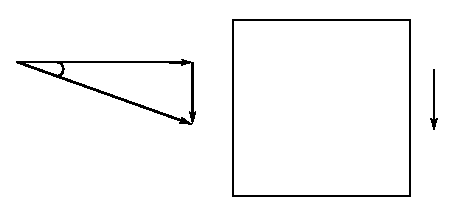
\includegraphics[width=0.5\unitlength]{../FnP/gnuplot/setup-1.eps}}         
      
      
   
 	\put(0.315,0.93){$U$}
 	\put(0.3,0.84){$U_i$}
    \put(0.42,0.88){$\dot{y}$}
    \put(0.28,0.895){ $\theta$}
    \put(0.7,0.87){\small $(+)$}
      	

 	
 	 

     

  \end{picture}

 \caption{Induced angle of attack on the square prism due to the resultant of free-stream velocity of the fluid and transverse velocity of the body.}
    \label{fig:setup_1}
\end{figure}

In the QSS model, it is assumed that the force on the body at a given instantaneous incident angle $\theta$ (defined in figure \ref{fig:setup_1}) is the same as the mean force on a static body at the same incident angle, or angle of attack. The instantaneous value of $C_y$ is therefore determined by an interpolating polynomial based on the lift force data for flow over a stationary body at various $\theta$. For an oscillating body, $\theta$ is related to the  instantaneous transverse velocity of the body $\dot{y}$ as illustrated in figure \ref{fig:setup_1}. Therefore, $C_y$ can be written as a function of $\dot{y}$.

The order of the interpolation polynomial for the lift force data has varied from study to study. For  example a $7^{th}$ order polynomial was used in \cite{Parkinson1964} and $3^{rd}$ order polynomial was used in \cite{Barrero-Gil2009}. \cite{Ng2005} concluded that using a $7^{th}$ order polynomial is sufficient and a polynomial higher than that of $7^{th}$ order doesn't provide a significantly better result. Thus a $7 ^{th}$ order interpolating polynomial is used in this present study. As a result, $C_y(\theta)$ (noting that theta is proportional to $\dot{y}/U$) is defined as
\begin{equation}
\label{cy ploynomial}
C_y(\theta)=a_1\left(\frac{\dot{y}}{U}\right)+a_3\left(\frac{\dot{y}}{U}\right)^3+a_5\left(\frac{\dot{y}}{U}\right)^5+a_7\left(\frac{\dot{y}}{U}\right)^7.
\end{equation}

%\begin{equation}
%\label{modified_equation_of_motion}
%\ddot{y}+c^*\dot{y}+k^*y=\frac{1}{2}\rho U^2A
%\end{equation}

 It is expected that vortex shedding will be well correlated along the span and provide significant forcing at low \reynoldsnumber. \citet{Joly2012} introduced  an additional sinusoidal forcing function to the hydrodynamic forcing to model this. This enables the model to provide accurate predictions even at low mass ratios where galloping excitation is suppressed or not present. However, the strength of this additional forcing needs to be tuned in an \emph{ad hoc} manner, and it is not clear how this forcing should vary with the other system parameters. Therefore, a focus of this study is to identify the parameter space where unmodified QSS model predicts power transfer accurately, and to quantify the the error in the regions where it does not predict accurately. Therefore the additional sinusoidal forcing function is disregarded. Substituting the definition of the lift coefficient provided in equation (\ref{cy ploynomial}) into the equation of motion of equation (\ref{lift equation}) gives 
 
\begin{equation}
\label{final_equation_motion}
m\ddot{y}{+}c\dot{y}{+}ky{=}\frac{1}{2}\rho U^2 \mathcal {A} \Bigg(a_1\left(\frac{\dot{y}}{U}\right){+}a_3\left(\frac{\dot{y}}{U}\right)^3{+}a_5\left(\frac{\dot{y}}{U}\right)^5{+}a_7\left(\frac{\dot{y}}{U}\right)^7.
\end{equation}

This ordinary differential equation can be solved using standard time integration methods. In this study the fourth-order Runge-Kutta scheme built in to the MATLAB routine `ode45' was used to obtain the solutions. 

\subsection{Calculation of average power}

 The dissipated power due to the mechanical damping represents the power transferred to the body from the fluid, and is the ideal potential amount of harvested power output before losses in any power take-off system are included. Therefore, the mean power output can be given by
\begin{equation}
\label{power}
P_{mean}=\frac{1}{T}\int_{0}^{T}(c\dot{y})\dot{y} dt,
\end{equation}
where $T$ is the period of integration and $c$ is the mechanical damping constant. 

It should be noted that this quantity is equal to the work done on the body by the fluid, defined as
\begin{equation}
\label{power_alt}
P_{mean}=\frac{1}{T}\int_{0}^{T}F_y\dot{y} dt,
\end{equation}
where $F_y$ is the transverse (lift) force.

These two definitions show two important interpretations of the power transfer. The first shows that power is a proportional to the mechanical damping and the magnitude of the transverse velocity. It is therefore tempting to think that the damping should be increased to increase the power transfer. In a power extraction device, the damping would be due to elctric generator, and an increased damping would be due to an increased electrical resistance or load. However, very high damping will have the effect of reducing the velocity amplitude. Because of this, a balance needs to be found where the damping is high, but not so high that it overly suppresses the motion of the body.

The second shows that power will be high for situations where the transverse force and the body velocity are in phase. Therefore, simply increasing the magnitude of the force or velocity is not sufficient to increase the power transfer, if this increase in magnitude is linked to an increase in phase.
 
\subsection{Parameters used} 
  
For the low \reynoldsnumber\ tests, a value of $\reynoldsnumber=200$ was used. Stationary $C_y$ data were obtained at different angles of attack ranging from $0^\circ$ to $16^\circ$. The average power was obtained by using equation \ref{power}, and the averaging was done over no less than 20 galloping periods. For the high \reynoldsnumber\ tests, predictions of power output at $\reynoldsnumber=22300$ were obtained using the coefficients for the $C_y$  curve from \citet{Parkinson1964} (Table (\ref{table:cy-coefficients})), in order to provide a comparison between high and low Reynolds numbers. The mass ratio $m^*$ was kept at 1163 for $\reynoldsnumber=22300$ (Similar to \citet{Parkinson1964}) and $m^*=20$ for \reynoldsnumber=200. These parameters were used throughout this study unless otherwise specified. 
 
The stationary data for the low \reynoldsnumber\ case and the DNS simulations of the fluid-structure interaction (FSI) problem were obtained using a high-order spectral element code to simulate the two-dimensional laminar flow. For all cases, a rectangular domain was employed where the inlet was placed $20D$ from the centre of the body, while the outlet was situated $60D$ away from the centre of the body. The lateral boundaries were placed $20D$ away from the centre of the body. The Navier--Stokes equations were solved in an accelerated frame of reference attached to the moving body, along with the body equation of motion given in equation \ref{equationofmotion}. A three-step time splitting scheme was used for the time integration. A time-dependent Dirichlet boundary condition was employed for the velocity on the inlet and lateral boundaries where $u=U$ and $v=-\dot{y}$ are the velocities in the $x$ and $y$ directions, respectively. A no-slip condition was enforced on the surface of the body. A Neumann condition, where the velocity gradient in the $x$ direction was set to zero, was enforced on the outlet. A Neumann condition for the pressure, where the normal gradient was calculated from the Navier--Stokes equations, was employed on the inlet, lateral and body surface \citep{gresho1987}, while a Dirichlet condition for the pressure ($p=0$ was enforced at the outlet. The details of the method can be found in \citet{Thompson2006,Thompson1996a}, and a description of the spectral element method in general can be found in \citet{karniadakis2005}. This code has been very well validated in a variety of fluid-structure interaction problems similar to that studied in this paper \citep{Leontini2007a,Griffith2011,Leontini2011,Leontini2013}.
  
The computational domain consists of 751 quadrilateral macro elements where the majority of the elements were concentrated near the square section. A freestream condition was given to the inlet, top and bottom boundaries and the normal velocity gradient was set to zero at the outlet. A convergence study was performed by changing the order of the polynomial ($p$-refinement) at $U^*=40$ and $\reynoldsnumber=200$. A $9^{th}$ order polynomial together with a time step of $\Delta tU/D=0.001$ was sufficient to ensure an accuracy of $2\%$ with regards to amplitude of oscillation.
  
\section{Results}
\label{sec:results}
  
\subsection{Static body results}
Figure \ref{fig:lift_curves} shows the plots $C_y$ as a function of $\theta$, as well as the interpolation polynomials. For high \reynoldsnumber\ the polynomial incorporated by \cite{Parkinson1964} was used. For low \reynoldsnumber\ two polynomials were used to obtain a better fit to the data. The first was fitted to the data $\theta=0^{\circ} \rightarrow 7^{\circ}$ and the second was fitted to the data $\theta > 7^{\circ}$. The coefficients of these polynomial fits are shown in table \ref{table:cy-coefficients}.

\begin{figure}

  \setlength{\unitlength}{\textwidth}
  \begin{picture}(1,0.25)(0,0.8)
  
    % % %90
      \put(0.025,0.81){\includegraphics[width=0.5\unitlength]{./chapter-pi_1_pi_2/FnP/gnuplot/lift_curve_200.eps}}
      \put(0.495,0.81){\includegraphics[width=0.5\unitlength]{./chapter-pi_1_pi_2/FnP/gnuplot/lift_curve_park.eps}}
 	\put(0.02,0.93){ \large $C_y$} 	
% 	\put(0.56,1.02){ $\theta$}
 	
        \put(0.25,0.8){ $\theta$} 	
        \put(0.75,0.8){ $\theta$}
        
        \put(0.117,1.01){(a)}
        \put(0.565,1.01){(b)}
      \end{picture}

  \caption{Lift coefficient, $C_y$, as a function of incidence angle $\theta$, for a static square cross section. (a) Data from simulations at $Re=200$  (b) data from \cite{Parkinson1964} at $Re=22300$. Points ($\bullet$) are measurements from the simulations. At $\reynoldsnumber=200$. Curves in both plots are 7th-order interpolating polynomials used to predict the fluid forcing for the QSS model. $C_y$ is the force coefficient of the force which occurs normal to the induced velocity.}
    \label{fig:lift_curves}
\end{figure}


\begin{table}[ht]

\begin{center}
\setlength{\unitlength}{\textwidth}

\begin{tabular}{c c c c c} % centered columns (4 columns)
\hline\hline %inserts double horizontal lines
\\[0.2ex]
Case & $a_1$ & $a_3$ & $a_5$ & $a_7$ \\ [0.8ex] % inserts table 
%heading
\hline 
\\[0.8ex]% inserts single horizontal line
Re=200 & 2.32 & 197.8 & 4301.7 & 30311.9 \\[0.8ex]% inserting body of the table
Re=22300 & 2.69 & 168 & 1670 & 59900 \\ [1ex] % [1ex] adds vertical space
\hline %inserts single line
\end{tabular}

\caption{Coefficient values used in the 7th order interpolation polynomial for high ($Re=22300$) and low ($Re=200$) Reynolds numbers. These data are used as input data to calculate the right-hand side of Eq. \ref{final_equation_motion} throughout this study.}
 
\label{table:cy-coefficients} % is used to refer this table in the text
\end{center}
\end{table}



There are several differences that can be observed between high and low Reynolds number data. The peak value of $C_y$ is  significantly lower at $\reynoldsnumber=200$ ($C_y=0.12$ at $5^\circ$) compared to $\reynoldsnumber=22300$ ($C_y=0.57$ at $13^\circ$) . The inflection point present around $8^\circ$ for $\reynoldsnumber=22300$ is not present at $\reynoldsnumber=200$. This agrees with the findings of \cite{Luo2003}.  It was concluded by \cite{Luo2003} that hysteresis in the system response occurs due to the inflection point in the $C_y$ curve. Therefore hysteresis is not expected at $\reynoldsnumber=200$.
    
The range of incident flow angles where $C_y$ remains positive is narrow at $\reynoldsnumber=200$ ($0^\circ <\theta \leq$ $7^\circ$) compared to $\reynoldsnumber=22300$ ($0^\circ <\theta \leq 15^\circ$). This feature is what sustains galloping. Power is only transferred from the fluid to the supporting structure within this range of incident angles because fluid forces are acting in the direction of travel of, or in phase with, the oscillating body as demonstrated by equation \ref{power_alt}. Incident angles beyond this range actually suppress the galloping and power is transferred in the opposite direction, i.e; from body to fluid. Therefore due to the overall smaller $C_y$ and narrow range of angles where $C_y$ is positive for $\reynoldsnumber=200$ compared to $\reynoldsnumber=22300$, it is expected that the transferred power at $\reynoldsnumber=200$ is significantly lower than at $\reynoldsnumber=22300$.

 % % % % % % % % % % % % % % % % % % % % % % % % % % % % % % % % % %
 \subsection{Formulation of the new dimensionless groups \massstiff \ and \massdamp}
\label{sec:newvar}
  The natural time scales of the system can be found by solving for the eigenvalues of the linearised equation of motion, namely
 \begin{equation}
 \label{eqn:eom_linear}
 m\ddot{y}{+}c\dot{y}{+}ky{=}\frac{1}{2}\rho U^2 \mathcal{A} a_1\left(\frac{\dot{y}}{U}\right),
 \end{equation}
 which is a simplified version of the equation of motion presented in equation \ref{final_equation_motion} with the polynomial series for the lift force truncated at the linear term.
 
Combining the $\dot{y}$ terms and solving for eigenvalues gives
 \begin{equation}
   \label{eqn:eigs}
   \lambda_{1,2}= -\frac{1}{2}\frac{c-\frac{1}{2}\rho U\mathcal{A}a_1}{m}\pm\frac{1}{2}\sqrt{\left[\frac{c-\frac{1}{2}\rho U\mathcal{A}a_1}{(m)}\right]^2-4\frac{k}{m}}.
 \end{equation}
 
If it is assumed that the spring is relatively weak, $k\rightarrow 0$, a single non-zero eigenvalue remains. This eigenvalue is
 \begin{equation}
   \label{eqn:eigs_nospring}
   \lambda=-\frac{c-\frac{1}{2}\rho U\mathcal{A}a_1}{m}.
 \end{equation}
 
Further, if it is assumed that the mechanical damping is significantly weaker than the aerodynamic forces on the body, $c\rightarrow 0$ and
 \begin{equation}
   \label{eqn:eigs_nospring_nodamp}
   \lambda=\frac{\frac{1}{2}\rho U\mathcal{A}a_1}{m}.
 \end{equation}
 

 In this form, $\lambda$ represents the inverse time scale of the motion of the body due to the effect of the long-time aerodynamic forces. In fact, the terms can be regrouped and $\lambda$ written as
 \begin{equation}
   \label{eqn:timescale}
   \lambda = \frac{a_1}{m^*}\frac{U}{D}
 \end{equation}
 
 Written this way, the important parameters that dictate this inverse time scale are clear. The rate of change in the aerodynamic force with respect to angle of attack when the body is at the equilibrium position, $\partial C_y/\partial \alpha$, is represented by $a_1$. The mass ratio is represented by $m^*$. The inverse advective time scale of the incoming flow is represented by the ratio $U/D$. Increasing $a_1$ would mean the force on the body would increase more rapidly with small changes in the angle of attack, $\theta$, or transverse velocity. Equation \ref{eqn:timescale} shows that such a change will increase the inverse time scale, or analogously decrease the response time of the body. Increasing the mass of the body, thereby increasing $m^*$, has the opposite effect. The inverse time scale is decreased, or as might be expected, a heavier body will respond more slowly.
 
This timescale can then be used to non-dimensionalize the equation of motion, and to find the relevant dimensionless groups of the problem. If the non-dimensional time, $\tau$, is defined such that $\tau=t(a_1/m^*)(U/D)$, the equation of motion presented in equation \ref{final_equation_motion} can be non-dimensionalized as
 \begin{equation}
   \label{eqn:eom_nondim}
   \ddot{Y} + \frac{m^{*2}}{a_1^2}\frac{kD^2}{mU^2}Y = \left(\frac{1}{2} - \frac{m^*}{a_1}\frac{cD}{mU}\right)\dot{Y} - \frac{a_1A_3}{m^{*2}}\dot{Y}^3 + \frac{a_1^3a_5}{m^{*4}}\dot{Y}^5 - \frac{a_1^5a_7}{m^{*6}}\dot{Y}^7.
 \end{equation}
 
The coefficients can be regrouped into combinations of non-dimensional groups, and rewritten as
 \begin{equation}
   \label{eqn:eom_nondim_regroup}
   \ddot{Y} + \frac{4\pi^{2}m^{*2}}{U^{*2}a_1^2}Y = \left(\frac{1}{2} - \frac{c^*m^*}{a_1}\right)\dot{Y} - \frac{a_1A_3}{m^{*2}}\dot{Y}^3 + \frac{a_1^3a_5}{m^{*4}}\dot{Y}^5 - \frac{a_1^5a_7}{m^{*6}}\dot{Y}^7,
 \end{equation}
where $U^{*}$ is the reduced velocity typically used as an independent variable in vortex-induced vibration studies and $c^*=cD/mU$ is a non-dimensional damping parameter.
 
Equation \ref{eqn:eom_nondim_regroup} shows there are five non-dimensional parameters that play a role in setting the response of the system. These are the stiffness (represented by the reduced velocity $U^*$), the damping $c^*$, the mass ratio $m^*$, and the geometry and \reynoldsnumber, represented by the coefficients of the polynomial fit to the $C_y$ curve, $a_n$. The grouping of these parameters into two groups in equation \ref{eqn:eom_nondim_regroup} which arise by non-dimensionalising using the natural time scale of the galloping system, suggests there are two groups that dictate the response: $\Gamma_1 = 4\pi^2m^{*2}/U^{*2}a_1^2$ and $\Gamma_2 = c^*m^*/a_1$. For a given geometry and Reynolds number, $\Gamma_1$ can be thought of as a combined mass-stiffness, whereas $\Gamma_2$ can be thought of a a combined mass-damping parameter. As it is assumed that during galloping the stiffness plays only a minor role, $\Gamma_2$ seems a likely parameter to collapse the data. In fact, in the classic paper on galloping from \cite{Parkinson1964}, galloping data from wind tunnel tests is presented in terms of a parameter that can be shown to be the same as $\Gamma_2$.
 
 All of the quantities that make up $\Gamma_1$ and $\Gamma_2$ can, in theory, be known before an experiment is conducted. However, the quantity $a_1$ is a relatively difficult one to determine, requiring static body experiments or simulations. Here, the geometry is unchanged and results are only being compared at the same \reynoldsnumber. Hence, suitable parameters can be formed by multiplying $\Gamma_1$ and $\Gamma_2$ by $a_1^2$ and $a_1$ respectively, to arrive at a mass-stiffness parameter $\massstiff =  4\pi^2m^{*2}/U^{*2}$, and a mass-damping parameter defined as $\massdamp = c^*m^*$.
 
 % % % % % % % % % % % % % % % % % % % % % % % % % % % % % % % % % % % % % % % % % % % % % % %
 \subsection{Comparison of \massstiff \ and \massdamp \ with classical VIV parameters}
\label{sec:new_vs_viv}

Another fluid-structure interaction phenomenon, vortex-induced vibration (VIV), has also been investigated as a candidate for the power extraction from flows. The work from \citet{Bernitsas2008a-concept, Bernitsas2009, Raghavan2010a, Lee2011b} and others from the same group at the University of Michigan have made significant progress with this problem. Therefore it may seem, at least initially, reasonable to present data from the fluid-elastic problem in the same parameters as typically used in VIV studies.
  
Figure \ref{fig:compare_data} shows the comparison of mean power data at $\reynoldsnumber=200$ presented using different independent variables. Subfigures (a), (c) and (e) show the displacement amplitude, velocity amplitude and the mean power as a function of the classic VIV parameter, \ustar for various damping ratios $\zeta$. Subfigures (b), (d) and (f) shows the same data as a function of \massdamp, for various, reasonably high values of \massstiff, as defined above in section \ref{sec:newvar}. The data presented using the classical VIV parameters follows the same trends as \cite{Barrero-Gil2010a}. However, the data presented using the dimensionless group formulated using the natural time scales of the system shows an excellent collapse for both velocity amplitude and mean power, showing that the power is essentially dictated by \massdamp. This implies that unlike VIV which is a type of resonant phenomenon, the natural frequency of the system which is used to scale \ustar, $\zeta$ and \massstiff\ does not have a large influence on the system behaviour in these cases.

\begin{figure}
  \setlength{\unitlength}{\textwidth}
  \fbox{
  \begin{picture}(1,0.9)(0,0)
    % % %90
      % % % Parkinson Data 
      \put(0.035,0.5){\includegraphics[width=0.5\unitlength]{../FnP/gnuplot/displacement_amp_re200.eps}}
      \put(0.035,0.27){\includegraphics[width=0.5\unitlength]{../FnP/gnuplot/velocity_amp_re200.eps}}
      \put(0.035,0.02){\includegraphics[width=0.5\unitlength]{../FnP/gnuplot/mean_power_re_200.eps}}
      
      \put(0.495,0.27){\includegraphics[width=0.5\unitlength]{../FnP/gnuplot/velocity_amp_collapsed_re200.eps}} 
      \put(0.495,0.02){\includegraphics[width=0.5\unitlength]{../FnP/gnuplot/mean_power_collapsed_re_200.eps}}
      \put(0.495,0.5){\includegraphics[width=0.5\unitlength]{../FnP/gnuplot/displacement_amp_collpased_re200.eps}}
      
%      \put(0.23,0.00){ $\displaystyle\frac{c}{\rho\mathcal{A}U}$}
%      \put(0.73,0.00){ $\displaystyle\frac{c}{\rho\mathcal{A}U}$}

      \put(0.28,0.00){\ustar}
      \put(0.78,0.00){\massdamp}
      
      \put(0.01,0.405){$\displaystyle\frac{V}{D}$}\
       \put(0.01,0.63){$\displaystyle\frac{A}{D}$}
      
      \put(-0.02,0.13){$\displaystyle\small\frac{P_{m}}{\rho \mathcal{A}U^3 }$}
      
      \put(0.093,0.705){\small(a)}
      \put(0.555,0.705){\small(b)}
      \put(0.093,0.475){\small(c)}
      \put(0.555,0.475){\small(d)}
      \put(0.093,0.225){\small(e)}
      \put(0.555,0.225){\small(f)}

  \end{picture}
}
  \caption{Displacement amplitude, velocity amplitude and mean power data as functions of two different independent varibles. Data presented in (a), (c) and (e) using the classical VIV parameter $\ustar$, obtained at $Re=200$ and $m^*=20$ at three different damping ratios: $\zeta=0.075$ ($\times$), $\zeta=0.1$ (\ding{117}) and $\zeta=0.15$ (+). (b) (d) and (f)  are the same data presented using the combined mass-damping parameter (\massdamp) as the independent variable.  }
  \label{fig:compare_data}
\end{figure}
    
\subsection{Comparison of power between high and low \reynoldsnumber data}   
\label{sec:low_vs_high_re}
The marked success of the collapse using \massdamp\ for the $\reynoldsnumber = 200$ case, particularly of the mean power, could also be replicated for the higher \reynoldsnumber\ case at $\reynoldsnumber = 22300$. Figure \ref{fig:collapsed_data} presents the mean power for both the high and low \reynoldsnumber\ cases for selected values of \massstiff. It is shown that the data collapse in both cases, demonstrating the validity of using \massdamp\ as an independent variable. \JL{Kasun: do you have data at different \massstiff\ for the high \reynoldsnumber\ case? You should include it here to show that the data collapses using \massdamp}

% !TeX spellcheck = en_GB
\begin{figure}
  \setlength{\unitlength}{\textwidth}

        \begin{picture}(1,0.3)(-0.02,0)

      % % % Parkinson Data 
%      \put(0.025,0.5){\includegraphics[width=0.5\unitlength]{../FnP/gnuplot/displacement_amp_collapsed_parkinson.eps}}
%      \put(0.025,0.27){\includegraphics[width=0.5\unitlength]{../FnP/gnuplot/velocity_amp_collapsed_parkinson.eps}}
%      \put(0.495,0.27){\includegraphics[width=0.5\unitlength]{../FnP/gnuplot/velocity_amp_collapsed_re200.eps}}
      
      \put(0.025,0.02){\includegraphics[width=0.5\unitlength]{../FnP/gnuplot/mean_power_collapsed_parkinson.eps}}
      \put(0.495,0.02){\includegraphics[width=0.5\unitlength]{../FnP/gnuplot/mean_power_optimum_re_200.eps}}
%      \put(0.495,0.5){\includegraphics[width=0.5\unitlength]{../FnP/gnuplot/displacement_amp_collpased_re200.eps}}
      
%      \put(0.23,0.00){ $\displaystyle\frac{c}{\rho\mathcal{A}U}$}
%      \put(0.73,0.00){ $\displaystyle\frac{c}{\rho\mathcal{A}U}$}

      \put(0.28,0.00){\massdamp}
      \put(0.74,0.00){\massdamp}
      
     
       \put(-0.03,0.13){$\displaystyle\frac{P_{m}}{\rho \mathcal{A}U^3 }$}
      

      \put(0.095,0.218){\small(a)}
      \put(0.565,0.218){\small(b)}
      
    \end{picture}

  \caption{Mean power as a function of \massdamp. Data presented at (a) $\reynoldsnumber=22300$, $\massstiff=200$ ($\times$), $massstiff=2000$ (\ding{117}) and $\massstiff=10000$ (+). (b) $\reynoldsnumber=200$, $\massstiff=100$. Hysteresis could be observed at high \reynoldsnumber  }
    \label{fig:collapsed_data}
\end{figure}

 %vspace{10cm}

         
Hysteresis could be observed for the $\reynoldsnumber = 22300$ case. The different solutions could be obtained by manipulating the initial conditions (initial displacement) of the system. The upper branch was obtained by giving an initial displacement which was higher than the expected amplitude while the lower branch was obtained by providing a lower initial displacement than the expected amplitude. Although theory shows a possible third state, it is an unstable branch and as such it could not be achieved numerically. This was also observed by \cite{Vio2007}. 

\subsection{Dependence on mass-stiffness, \massstiff}
\label{sec:massstiff}

The results of sections \ref{sec:new_vs_viv} and \ref{sec:low_vs_high_re} show that the mean extracted power is essentially a function of a single variable, the combined mass-damping \massdamp. However, the timescale analysis of section \ref{sec:newvar} showed that a second variable, the combined mass-stiffness \massstiff\ should also play a role. Here, the impact of this variable is investigated further. Overall, the system behaviour can be separated into two wide regimes; that for ``high'' \massstiff\ and that for ``low'' \massstiff. These two regimes are further investigated and explained in this following section.

Figure \ref{fig:high_pi_1} shows the mean power as a function of \massdamp\ for a range of values of \massstiff. Two subfigures are shown; subfigure (a) shows data for $\massstiff \geq 10$, while (b) shows data for $\massstiff \leq 10$. In figure \ref{fig:high_pi_1}(a), the collapse of the mean power is excellent, showing that for $\massstiff \geq 10$, the mean power is independent of \massstiff.

\begin{figure}
  \setlength{\unitlength}{\textwidth}
\fbox{
        \begin{picture}(1,1.1)(0,0.35)

      % % % Parkinson Data 
      \put(0.09,1.1){\includegraphics[width=0.757\unitlength]{../FnP/gnuplot/displacement_high_pi_1.eps}}
      \put(0.1,0.75){\includegraphics[width=0.75\unitlength]{../FnP/gnuplot/velocity_high_pi_1.eps}}
      \put(0.1,0.35){\includegraphics[width=0.75\unitlength]{../FnP/gnuplot/mean_power_high_pi_1.eps}}
      
         \put(0.07,0.95){$\displaystyle\frac{V}{D}$}\
         \put(0.07,1.3){$\displaystyle\frac{A}{D}$}
         \put(0.05,0.6){$\displaystyle\frac{P_{m}}{\rho \mathcal{A}U^3 }$}



%      
%      \put(0.45,0.7){\small(a)}
%      \put(0.926,0.7){\small(b)}
%      \put(0.726,0.45){\small(c)}
%  

      
    \end{picture}
}
  \caption{QSS data at high \massstiff \ levels. (a) displacement amplitude, (b) velocity amplitude and (c) mean power as a function of \massdamp. Data presented at four different combined mass-stiffness levels.\ $\massstiff=10 \ (\mstar=20,\ \ustar \approx 40)$ \ (\ding{117}),\ $\massstiff=100 \ (\mstar=130,\ \ustar \approx 80) \ (+)$ and \ $\massstiff=1000 \ (\mstar=400,\ \ustar \approx 40) \ (\triangle)$}
    \label{fig:high_pi_1}
\end{figure}

 %vspace{10cm}


For low values of $\massstiff \leq 10$, figure \ref{fig:high_pi_1}(b) shows that the predicted mean power increases as \massstiff\ is decreased, indicating that the mean power is a weak function of \massstiff\ at low \massstiff\ levels. This provides the distinction between high and low \massstiff\ regimes. For high values where $\massstiff \geq 10$, the mean extracted power is a function of \massdamp\ only; for low values where $\massstiff < 10$, the mean extracted power is a weak function of \massstiff.

Regardless of the value of \massstiff, the variation of the mean extracted power with \massdamp\ is essentially the same. With increasing \massdamp, the mean extracted power initially increases, before reaching some maximum value and then decreasing. This relationship between power and \massdamp\ can be explained by analysing the time histories of selected cases. Data at $\massstiff=10$, $m^*=20$ and $\reynoldsnumber=200$ are shown in figure \ref{fig:power_time_histories} and are analysed as an example. Values of \massdamp\ less than (region 1), equal to (region 2), and greater than (region 3) the value where the mean extracted power is a maximum are analysed as examples.

\begin{figure}

  \setlength{\unitlength}{\textwidth}
%  \fbox{
  \begin{picture}(1,0.58)(0,0.35)
    % % % 90
    \put(0.03,0.76){\includegraphics[width=0.35\unitlength]{../FnP/gnuplot/power_time_history_015.eps}}
    \put(0.03,.58){\includegraphics[width=0.35\unitlength]{../FnP/gnuplot/f_y_history_015.eps}}
    \put(0.03,0.4){\includegraphics[width=0.35\unitlength]{../FnP/gnuplot/theta_time_history_015.eps}}
    
    % % 165
    \put(0.36,0.76){\includegraphics[width=0.35\unitlength]{../FnP/gnuplot/power_time_history_54.eps}}
    \put(0.36,.58){\includegraphics[width=0.35\unitlength]{../FnP/gnuplot/f_y_history_54.eps}}
    \put(0.36,0.4){\includegraphics[width=0.35\unitlength]{../FnP/gnuplot/theta_time_history_54.eps}}
    
    \put(0.68,0.76){\includegraphics[width=0.35\unitlength]{../FnP/gnuplot/power_time_history_08.eps}}
    \put(0.68,.58){\includegraphics[width=0.35\unitlength]{../FnP/gnuplot/f_y_history_08.eps}}
    \put(0.68,0.4){\includegraphics[width=0.35\unitlength]{../FnP/gnuplot/theta_time_history_08.eps}}
    
    \put(0.55,0.36){$\displaystyle{\frac{tU}{D}}$}
    \put(0.2,0.36){$\displaystyle{\frac{tU}{D}}$}
    \put(0.85,0.36){$\displaystyle{\frac{tU}{D}}$}
    
    \put(0.0,0.87){$\frac{P}{\rho \mathcal{A}U^3}$}
    \put(0.01,0.66){$F_y$}
    \put(0.01,0.49){$\theta$}
    
    \put(0.08,0.76){(a)}
    \put(0.08,0.58){(d)}
    \put(0.08,0.38){(g)}
    
    \put(0.4,0.76){(b)}
    \put(0.4,0.58){(e)}
    \put(0.4,0.38){(h)}
    
    \put(0.72,0.76){(c)}
    \put(0.72,0.58){(f)}
    \put(0.72,0.38){(i)}
  \end{picture}
%}
  \caption{Time histories of $P_t$, $P_d$, $F_y$ and $\theta$ at $\massdamp=0.15$, $0.54$ and $0.8$ from the QSS model. Data was obtained at $m^*=20$, $\massstiff=10$ and \reynoldsnumber=200. The time histories of $P_t$ ( \solidrule[4mm]\hspace{1mm}) and $P_d$ (\protect\dashedrule) are presented for: (a) $\massdamp= 0.15$; (b) $\massdamp= 0.54$; (c) $\massdamp= 0.8$. Time histories of the instantaneous force $F_y$ for: (d) $\massdamp= 0.15$; (e) $\massdamp= 0.54$; (f) $\massdamp= 0.8$. Time histories of the instantaneous angle $\theta$ for: (g) $\massdamp= 0.15$; (h) $\massdamp= 0.55$; (i) $\massdamp= 0.8$.}
  \label{fig:power_time_histories}
\end{figure}






The instantaneous power from the fluid to the body can be expressed as $P_t=F_y\dot{y}$. Similarly the dissipated power due to the mechanical damping can be expressed as $P_d=(c\dot{y})\dot{y}$. The time average of these two quantities, described in equations \ref{power} and \ref{power_alt} must be equal due to energy conservation.
 
% Figure \ref{fig:lift_curves}(a) shows that $C_y$ and therefore instantaneous force rises until $4^\circ$ where it peaks and then falls, and at around $6^\circ$ becomes negative. The maximum instantaneous power that can be transferred occurs when $C_t\dot{y}$ is a maximum which occurs when $\theta$ is close to the peak in the $C_y$  curve . At the region where the instantaneous force becomes negative it will be opposing the velocity $\dot{y}$. 
 
 % % % % % % % % % % % don  

At region 1 ($\massdamp=0.3$) the damping is low in comparison with region 2 and 3. While this may lead to larger oscillations, damping is required to dissipate and therefore extract power according to equation \ref{power}. Therefore, the low damping in this region leads to a low mean power output. Fig.\ref{fig:power_time_histories} (a) shows that $P_d$ (the power dissipated by damping) becomes negative over some portion of the cycle. This is caused by the high velocity amplitude leading to the equivalent incident angle $\theta$ to exceed the range where $C_y$ is positive (i.e. $0<\theta<6^\circ$ as shown in figure\ref{cy ploynomial}(a)). In this portion of the cycle the fluid-dynamic force actually opposes the direction of travel and power is transferred from the structure to the fluid during those times. From an energy perspective, the mechanical damping is not sufficient to remove the energy transferred from the fluid to the structure through work during other times of the cycle because $\massdamp$ \ is substantially low. Therefore this excess energy is transferred back to the fluid as depicted by the negative region of $P_d$.
 
At region 3 where $\massdamp=0.8$ the damping constant is high and a clear sinusoidal signal is observed for both $P_d$ and $P_t$ in figure \ref{fig:power_time_histories}(c). Figures \ref{fig:power_time_histories}(f) and  \ref{fig:power_time_histories}(i) show that equivalent incident angle $\theta$ (which for small values, is proportional to the transverse velocity of the body) is in phase with $F_y$.  The velocity amplitude in this case is small and $\theta$ is within the range where the hydrodynamic force increases with the incident angle (i.e. $0<\theta \leq 5^\circ$ as shown in figure \ref{fig:lift_curves}(a)). According to equation \ref{power_alt}, these conditions are suitable for high power output. However in this case, the high damping limits the velocity amplitude and results in relatively low fluid dynamic forces.
  
At region 2 ( $\massdamp=0.54$), a balance is found between high and low values of damping. $P_d$ is not a pure sinusoidal signal, however the signal remains periodic. From the time history graph of $P_d$, two `peaks' are present in a single half cycle as shown in figure \ref{fig:power_time_histories}(b). In this case, the velocity amplitude actually exceeds the equivalent incident angle where the hydrodynamic forces peaks (i.e. $\theta=5^\circ$ in \ref{cy ploynomial} (a)). The dips in $P_d$ between the two peaks approximately correspond to the time where the transverse velocity is higher than 0.09 and $F_y$ is decreasing with increasing transverse velocity. The mean power output is at its maximum. This is due to the fact that this region is the best compromise between region 1 and 3. The damping is high enough to obtain a high power output while not so high that the motion is completely suppressed.

\subsection{Dependence on the mass ratio \mstar}
\label{sec:mstar}
While for high values of \massstiff\ it is clear that the mean extracted power is a function of \massdamp\ only, a question arises for low values of \massstiff; is the variation in the mean extracted power purely a function of \massstiff, or is it also a function of the mass ratio \mstar? To answer this question, the model has been solved for a fixed value of \massstiff, but for varying values of \mstar. This means that \massstiff\ was varied by changing the system stiffness.

Figure \ref{fig:low_pi_1} shows the mean extracted power as a function of \massdamp, for a fixed $\massstiff = 0.1$, for three different values of \mstar. From the figure it is clear that the results are independent of \mstar, and are a function of \massstiff\ and \massdamp\ only.

\begin{figure}
  \setlength{\unitlength}{\textwidth}

        \begin{picture}(1,0.4)(0,0.4)

      % % % Parkinson Data 
%      \put(0.1,1.1){\includegraphics[width=0.75\unitlength]{../FnP/gnuplot/displacement_low_pi_1.eps}}
%      \put(0.1,0.76){\includegraphics[width=0.75\unitlength]{../FnP/gnuplot/velocity_low_pi_1.eps}}
      \put(0.1,0.42){\includegraphics[width=0.75\unitlength]{./chapter-pi_1_pi_2/FnP/gnuplot/mean_power_low_pi_1.eps}}
      
%       \put(0.07,0.95){$\displaystyle\frac{V}{D}$}
%       \put(0.07,1.3){$\displaystyle\frac{A}{D}$}
       \put(0.05,0.6){$\displaystyle\frac{P_{m}}{\rho \mathcal{A}U^3 }$}
       \put(0.5,0.4){$\massdamp$}
       \
%\put(0.189,1.415){\small(a)}
%\put(0.189,1.07){\small(b)}
%\put(0.189,0.73){\small(c)}

%  

      
    \end{picture}

  \caption{Dimensionless mean power as a function of \massdamp\ obtained using QSS model at \ $\massstiff=0.1$.  Data presented at  $\mstar=2$ (\ding{117}), \  $ \mstar=20 \ (\triangle)$ and  $ \mstar=50 \ (*)$. The mass ratio does not have an effect on \massstiff \ even at low \massstiff.}
    \label{fig:low_pi_1}
\end{figure}

 %vspace{10cm}

 
\subsection{Comparison with DNS data}
\label{sec:dns}

The QSS model assumes that the only force driving the system is the instantaneous lift generated by the induced velocity. However, vortex shedding is also present in this system. Therefore, an essential assumption when this model is used, is that the effect of vortex shedding is minimal. Hence, the model has been always used at high \reynoldsnumber \ and  at high mass ratios. The present study is focused on identifying the limiting parameters of the QSS model at low Reynolds numbers by providing a comparison with DNS results. 

\citet{Joly2012} showed that the displacement data obtained using the QSS assumption and DNS agree well at low Reynolds numbers, with the modification implemented to the oscillator equation which accounts for the vortex shedding. These data were obtained at zero damping levels. However, the current study is focused on the behaviour and the power transfer of the system. Therefore analysing the behaviour of the system with increasing damping is of interest.

The comparison between QSS and the DNS results is presented in figure \ref{fig:qss_fsi}. The maximum displacement, velocity and mean extracted power are presented as a function of \massdamp. A range of values of \massstiff\ are compared to the QSS model data for $\massstiff = 10$. Figures \ref{fig:qss_fsi}(a) and \ref{fig:qss_fsi}(b) show little variation with \massstiff, and the comparison between the QSS model and the DNS simulations is quite good. However, the mean extracted power shown in figure \ref{fig:qss_fsi}(c) reveals that the mean power is influenced by both \massstiff\ and \massdamp. This is particularly clear for low values of \massstiff, where the discrepancly between the QSS model predictions of power and the DNS simulations is the largest. Comparing figure \ref{fig:qss_fsi}(c) with figure \ref{fig:high_pi_1}(b) shows that \massstiff has much more influence on the power extracted than predicted by the QSS model. In fact, the QSS model predicts that the mean extracted power should increase with decreasing \massstiff, whereas the DNS simulations show that the mean extracted power decreases with decreasing \massstiff.

\begin{figure}
  \setlength{\unitlength}{\textwidth}

        \begin{picture}(1,1.1)(0,0.35)

      % % % Parkinson Data 
      \put(0.1,1.1){\includegraphics[width=0.75\unitlength]{./chapter-pi_1_pi_2/FnP/gnuplot/fqss_fsi_displace.eps}}
      \put(0.1,0.737){\includegraphics[width=0.75\unitlength]{./chapter-pi_1_pi_2/FnP/gnuplot/qss_fsi_velocity.eps}}
      \put(0.1,0.38){\includegraphics[width=0.75\unitlength]{./chapter-pi_1_pi_2/FnP/gnuplot/qss_fsi_power.eps}}
      
      



%      
    \put(0.15,1.41){\small(a)}
     \put(0.15,1.05){\small(b)}
     \put(0.15,0.69){\small(c)}
\put(0.03,0.95){$\displaystyle\frac{V}{U}$}
\put(0.03,1.3){$\displaystyle\frac{A}{D}$}
\put(0.0,0.56){$\displaystyle\frac{P_{m}}{\rho \mathcal{A}U^3 }$}
\put(0.466,0.35){$\massdamp$}

      
    \end{picture}

    \caption{Comparison of data generated using the quasi-static model
      and full DNS simulations at (a) Displacement amplitude, (b)
      velocity amplitude and (c) dimensionless mean power as functions of
      \massdamp. Data were obtained at $\reynoldsnumber = 200$ at four
      values $\massstiff=10$ ($\mstar= 20.13$) (\ding{83}),
      $\massstiff=60$ ($\mstar =49.31$) (\ding{108}), $\massstiff=250$
      ($\mstar= 100.7$) ($\triangle$) and $\massstiff=1000$ ($\mstar=201.3$) (\ding{117}). The QSS data at $\massstiff=10$ \
      (\protect\dashedrule).}
    \label{fig:qss_fsi}
\end{figure}

 %vspace{10cm}


Figure \ref{fig:max_power}(a) clearly shows the dependence of the mean extracted power on \massstiff. Here, the maximum power extracted for a given value of \massstiff, over all values of \massdamp (essentially the value of extracted power at the turning point), is plotted as a function of \massstiff. These values were obtained by fitting a quadratic to the data of figure \ref{fig:low_pi_1} and finding the value of mean extracted power at the turning point. The rapid decrease in the extracted power as $\massstiff \rightarrow 0$ is clear.

% !TeX spellcheck = en_GB
\begin{figure}
  \setlength{\unitlength}{\textwidth}
  \begin{picture}(1,0.3)(-0.02,0)
          
    \put(0.025,0.04){\includegraphics[width=0.45\unitlength]{../FnP/gnuplot/p_max.eps}}
    \put(0.54,0.04){\includegraphics[width=0.45\unitlength]{../FnP/gnuplot/p_2_p_max.eps}}
        
    \put(0.48,0.07){ \rotatebox{90}{$\displaystyle\massdamp$ \scriptsize{at max power}} }
    \put(-0.07,0.16){$\displaystyle\frac{P_{max}}{\rho \mathcal{A}U^3 }$}
    % \put(0.73,0.00){ $\displaystyle\frac{c}{\rho\mathcal{A}U}$}

    \put(0.24,0.00){\massstiff}
    \put(0.75,0.00){\massstiff}
   
    \put(0.058,0.07){\small(a)}
    \put(0.57,0.07){\small(b)}
      
    \end{picture}

    % \caption{Comparison of DNS data. (a) Maximum power obtained using
    %   a 3 point localised quadratic fitting as a function of
    %   \massstiff. (b) \massdamp as a function of \massstiff at maximum
    %   power}

    \caption{(a) Maximum power of QSS data ($\circ$) and DNS data ($\bullet$), and (b) the value of \massdamp\ 
        where maximum power occurs in DNS data, as functions of \massstiff.
           The maximum power asymptotes to an upper
        value with increasing \massstiff, while the value of \massdamp\
        where maximum power occurs is relatively insensitive to
        \massstiff. The maximum power of the DNS data remains relatively constant as shown before. The dash curve (\protect\dashedrule) of (a) follows the logarithmic fit of the maximum power which is $f(x)=1.48 \times 10^{-4} \ ln(x) + 1.9 \times 10^{-3} $ equation.}

    \label{fig:max_power}
\end{figure}

 %vspace{10cm}


Figure \ref{fig:max_power}(a) also shows that \massstiff\ is important to higher values than predicted by the QSS model. For the QSS model, the mean extracted power was essentially independent of \massstiff\ for $\massstiff>10$; however, the mean extracted power from the DNS data shows a significant dependence on \massstiff\ for $\massstiff<250$.

Figure \ref{fig:max_power}(b) shows the value of \massdamp\ at which the turning point, and therefore the maximum power output, occurs. It is shown that while the power extracted is a reasonably strong function of \massstiff, the value of \massdamp\ at which this maximum power occurs is relatively unaffected. 

In an effort to quantify the performance of the QSS model, the percentage between the QSS and DNS extracted power data as a function of \massstiff\ was calculated using the equation
 \begin{equation}   \label{eqn:error_calculation} 
 \% \ error=\left|{\frac{P_{m(QSS)} - P_{m(DNS)}}{P_{m(DNS)}}}\right| \times 100.
 \end{equation}

The results of this calculation are plotted in figure \ref{fig:error}, along with a power-law best fit \JL{Kasun put the formula for the power law fit here.}. The figure clearly shows that as \massstiff increases, the error between the QSS and DNS models quickly decreases. However, at low values of \massstiff, the discrepancy between the two can be quite large, around $30\%$.

\begin{figure}
  \setlength{\unitlength}{\textwidth}

        \begin{picture}(1,0.4)(0,0.4)

      \put(0.1,0.45){\includegraphics[width=0.75\unitlength]{../FnP/gnuplot/error.eps}}
      
%       \put(0.07,0.95){$\displaystyle\frac{V}{D}$}
%       \put(0.07,1.3){$\displaystyle\frac{A}{D}$}
       \put(0.05,0.58){\rotatebox{90}{$\% \ error$}}
%       \put(0.5,0.4){$\massdamp$}
       \put(0.5,0.4){$\massstiff$}
    \end{picture}

  % \caption{Comparison of maximum power between QSS and DNS data obtained using 3 point local quadratic curve fitting.The error was obtained using Eq:\ref{eqn:error_calculation}}
    \caption{The difference between the maximum power predicted by
        the QSS model for $\massstiff = 10$, and the DNS data as a
        function of \massstiff. The QSS model prediction is worst for
        low values of \massstiff.}
    \label{fig:error}
\end{figure}

 %vspace{10cm}


A likely reason for this discrepancy at low \massstiff\ is the influence of the vortex shedding, which is not accounted for in the QSS model. To investigate this further, frequency spectra for the body velocity from DNS cases at varying values of \massstiff, at a value of $\massdamp=0.47$ (close to the value at which the mean extracted power is a maximum), have been produced. They are presented, along with the original time histories in figure \ref{fig:spectrum}.

\begin{figure}
  \setlength{\unitlength}{\textwidth}

  \begin{picture}(1,1.2)(0,-0.1)
    % % %90
      % % % Parkinson Data 
      \put(0.005,0.8){\includegraphics[width=0.5\unitlength]{../FnP/gnuplot/spec_20_sig.eps}}
      \put(0.005,0.5){\includegraphics[width=0.5\unitlength]{../FnP/gnuplot/spec_50_sig.eps}}
      \put(0.005,0.27){\includegraphics[width=0.5\unitlength]{../FnP/gnuplot/spec_100_sig.eps}}
      \put(0.005,0.02){\includegraphics[width=0.5\unitlength]{../FnP/gnuplot/spec_200_sig.eps}}
      
      
      \put(0.505,0.8){\includegraphics[width=0.5\unitlength]{../FnP/gnuplot/spec_20.eps}}
      \put(0.505,0.5){\includegraphics[width=0.5\unitlength]{../FnP/gnuplot/spec_50.eps}}
      \put(0.505,0.27){\includegraphics[width=0.5\unitlength]{../FnP/gnuplot/spec_100.eps}} 
      \put(0.505,0.02){\includegraphics[width=0.5\unitlength]{../FnP/gnuplot/spec_200.eps}}
      
      
%      \put(0.23,0.00){ $\displaystyle\frac{c}{\rho\mathcal{A}U}$}
%      \put(0.73,0.00){ $\displaystyle\frac{c}{\rho\mathcal{A}U}$}

      \put(0.28,-0.03){$\displaystyle\frac{fd}{U}$}
      \put(0.78,-0.03){$\displaystyle\frac{tU}{D}$}
      
      \put(0.51,0.405){$\displaystyle\frac{V}{D}$}
      \put(0.51,0.63){$\displaystyle\frac{V}{D}$}
      \put(0.51,0.13){$\displaystyle\frac{V}{D}$}
      \put(0.51,0.93){$\displaystyle\frac{V}{D}$}
      
      \put(0.10,0.995){\small(a)}
      \put(0.625,0.995){\small(b)}
      \put(0.1,0.695){\small(c)}
      \put(0.625,0.695){\small(d)}
      \put(0.1,0.465){\small(e)}
      \put(0.625,0.465){\small(f)}
      \put(0.1,0.217){\small(g)}
      \put(0.625,0.217){\small(h)}

  \end{picture}

  \caption{Velocity signal (right) and the corresponding power spectrum (left) of the DNS data at 3 different \massstiff \ at $\massdamp=0.8$. (a) and (b) $\massstiff=10$, (c) and (d) $\massstiff=60$, (e) and (f) $\massstiff=250$, (g) and (h) $\massstiff=1000$. \ustar \ is kept at 40 therefore the mass ratio increases as \ \massstiff \ increases. It is evident that the influence of vortex shedding reduces as the inertia of the system increases.}
  \label{fig:spectrum}
\end{figure}
 
This figure shows the  velocity signals at $\massstiff=0.8$ and $\massdamp= 10, 60, 250$ and $1000$ and the corresponding spectrum. The spectral data shows a significant component around $fd/U=0.156$ which can be identified as the vortex shedding frequency. The magnitude of the component at the vortex shedding frequency clearly reduces as \massstiff\ is increased. This indicates that the influence of vortex shedding is much more prominent at low \massstiff,  therefore resulting in larger deviations from quasi-steady state results. This builds on the work of \cite{Joly2012}, which was conducted at zero damping, that implied that mean extracted power would be influenced by vortex shedding at low mass.

This influence is explicitly shown here. Figure \ref{fig:spec_pow} plots the relative intensity of the component at the vortex shedding frequency to the component at the galloping or oscillation frequency in the spectra of figure \ref{fig:spectrum}.

\begin{figure}
  \setlength{\unitlength}{\textwidth}

        \begin{picture}(1,0.4)(0,0.4)

      \put(0.1,0.45){\includegraphics[width=0.75\unitlength]{../FnP/gnuplot/spec_pow.eps}}
      
%       \put(0.07,0.95){$\displaystyle\frac{V}{D}$}
%       \put(0.07,1.3){$\displaystyle\frac{A}{D}$}
       \put(0.045,0.43){\rotatebox{90}{$relative \ power \ of \ shedding$ }}
%       \put(0.5,0.4){$\massdamp$}
       \put(0.43,0.4){$\massstiff$}
    \end{picture}

  % \caption{Comparison of maximum power between QSS and DNS data obtained using 3 point local quadratic curve fitting.The error was obtained using Eq:\ref{eqn:error_calculation}}
    \caption{The relative power of the vortex shedding as a fucntion of \massstiff. The relative power of the vortex shedding decreases as \massstiff \ increases. This trend follows $0.977x^{-0.5}$ equation}
    \label{fig:spec_pow}
\end{figure}

 %vspace{10cm}


Similar to the discrepancy between the QSS and DNS mean extracted power shown in figure \ref{fig:error}, the relative strength of the vortex shedding is seen to be large at small values of \massstiff, and quickly decreases as \massstiff\ is increased. This correlation strongly indicates this discrepancy is due to the influence of the vortex shedding, even though the vortex shedding and galloping frequencies remain separated by around the same amount for all values of \massstiff\ presented in figure \ref{fig:spectrum}. The data presented in figure \ref{fig:spec_pow} also give some indication of the strength of any vortex shedding correction term that might be added to the QSS model in an effort to decrease the discrepancy between it and the DNS simulations.


 
\section{Conclusion}
\label{sec:conc}
In this paper the power transfer of a square body under fluid-elastic galloping is analysed by solving the quasi-steady state oscillator model equation using numerical  integration. The QSS model provides equations where dimensionless groups could be formulated using the relevant time scales. A good collapse for predicted output of power could be obtained using these dimensionless groups in comparison with the classical VIV parameters i.e. $\zeta$ and \ustar. The collapsed data using the dimensionless groups strengthens the argument that the velocity amplitude and the power transfer of the system does not depend on the natural frequency of the system. 
  
In comparison with the direct numerical simulation data, it could be concluded that the QSS model provides a good estimate of the power output of the system when \massstiff\ is relatively high. However at low values of \massstiff, the prediction is not close due to the fact that the QSS model does not account for the impact of vortex shedding which is shown to increase in influence as \massstiff\ is decreased. However, the QSS model does provide a good prediction of the value of \massdamp\ at which maximum power is produced. The error in predicted maximum power between the QSS and the DNS data scales as an inverse function of \massdamp, similar to the scaling of the influence of the vortex shedding on the body velocity.
  
  
 
 
 
 
 
 
 
 
 
 
 
 
 
 
 
 
 
 
 
 
 
 
 
 
 
 







